\documentclass{article}%
\usepackage[T1]{fontenc}%
\usepackage[utf8]{inputenc}%
\usepackage{lmodern}%
\usepackage{textcomp}%
\usepackage{lastpage}%
\usepackage{authblk}%
\usepackage{graphicx}%
%
\title{Interleukin{-}1 b inhibits NaC{-}KCATPase activity and protein expression in cardiac myocytes}%
\author{Raymond Dominguez}%
\affil{Department of Laboratory Medicine, The First Affiliated Hospital of Sun Yat{-}sen University, Guangzhou, Guangdong, China}%
\date{01{-}01{-}2012}%
%
\begin{document}%
\normalsize%
\maketitle%
\section{Abstract}%
\label{sec:Abstract}%
SAN DIEGO {-} Results of a new epidemiology evaluation of the Salmonella enterica Type III secretion system effector (SLEAS) in the laboratory of Jose Luis Trinidad showed certain proteins to be effectively passed on from the cell to its host by the SLEAS influence.\newline%
This finding can be used as a valuable information point to support use of recombinant vaccines (RVs) to protect against deadly pathogens, and the importance of sanitation for minimizing such consequences.\newline%
Even if an SLEAS pure virus was not infecting a host cell, it could easily pass in and kill the host cell cell itself, explained John Snow, a biostatistician at the University of California, San Diego (UCSD) who conducted the study. Its a perfect recipe for a bad outcome, but we need to look at how to make it be better, and how we can help prevent it.\newline%
Individual diseases with strong chesnut{-}reproduction levels of a SLEASed carrier are rare and unlikely to be transmitted from cell to cell. However, those defects that can prevent the carriers from delivering a potent payload to cell can cause a serious health risk.\newline%
If you had the choice to prevent an inactivated virus from infecting you and your family or the infection, in the situation of a close friend or loved one, would you do what we tell patients when we discuss infectious disease risk? commented J. David Olsen, who co{-}authored the report published in Environmental Health Perspectives. Its a tough question. With the newest generation of recombinant vaccine, researchers are finding even more amazing, promising ways to prevent the spread of infectious disease.\newline%
The finding is significant, given that immune cells, microorganisms and DNA, are proteins involved in transmission to the host cell. While the discovery, if validated, could be added to existing research in virus replication and the ability of viruses to contaminate host cells, it is highly speculative until the evidence is in.\newline%
Further studies will evaluate how the SLEAS changes the ability of immune cells to differentiate and suppress the RNA of invading pathogens and how other cell functions affect the transmission of the protein changes to the host cell.\newline%
Researchers from UCSD, two U.S. Department of Homeland Security (DHS) Centers for Biomedical Advanced Research and Development Authority (CABRA) Centers for Pathogens (CAP{-}CR), and members of the North American Combustion Transplant Consortium also participated in the study.\newline%
The latest results are welcome news, however, as previous studies have shown that not only could antibodies from the cells not properly bind to and neutralize the SLEAS protein if the contaminant was detected, but the SLEAS and invaders have problems regulating the value of the immune response.

%
\subsection{Image Analysis}%
\label{subsec:ImageAnalysis}%


\begin{figure}[h!]%
\centering%
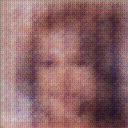
\includegraphics[width=150px]{500_fake_images/samples_5_356.png}%
\caption{A Close Up Of A Person Wearing A Tie}%
\end{figure}

%
\end{document}